\Large\textbf{\textcolor{blue}{4.}}
Observa la siguiente función del lenguaje de programación \code{Racket}.

\begin{lstlisting}
(let ([fib (lambda (n) (if (or (zero? n) (= n 1)) 1 (+ (fib (- n 1)) (fib (- n 2)))))])
      (fib 3))
\end{lstlisting}

\begin{enumerate}[a.]
%%%%%%%%%%%%%%%%%%%%%%%%%%%%%      Inciso A        %%%%%%%%%%%%%%%%%%%%%%%%%%%%%%%%%
\item Prueba la expresión en el intérprete de \code{Racket} y con base en la respuesta 
obtenida, explica el proceso que siguió el intérprete para llegar a ésta. Anexa una 
captura de pantalla del intérprete de \code{Racket} al probar la expresión.

\begin{figure}[h]
  \centering
  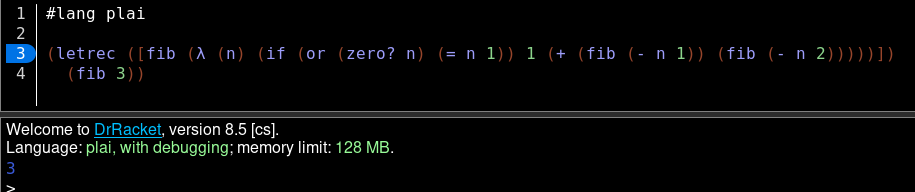
\includegraphics[scale=0.5]{./Fib.png}
  \caption{Ejecución de la función dada.}
\end{figure}

\begin{lstlisting}
> (let ([fib (lambda (n) (if (or (zero? n) (= n 1)) 1 (+ (fib (- n 1)) (fib (- n 2)))))])
      (fib 3))
= (+ (fib (- 3 1)) (fib (- 3 2)))
= (+ (+ (fib (- 2 1)) (fib (- 2 2))) (fib 1))
= (+ (+ (1) (1)) (1))
= (+ 2 1)
= 3
\end{lstlisting}
%%%%%%%%%%%%%%%%%%%%%%%%%%%%%      Inciso B        %%%%%%%%%%%%%%%%%%%%%%%%%%%%%%%%%
\item Modifica la función usando el Combinador de Punto Fijo Y .Prueba la expresión en 
el intérprete de \code{Racket} y con base en la respuesta obtenida, explica el proceso que 
siguió el intérprete para llegar a ésta. Anexa una captura de pantalla del intérprete 
de \code{Racket} al probar la expresión.

\begin{figure}[h]
  \centering
  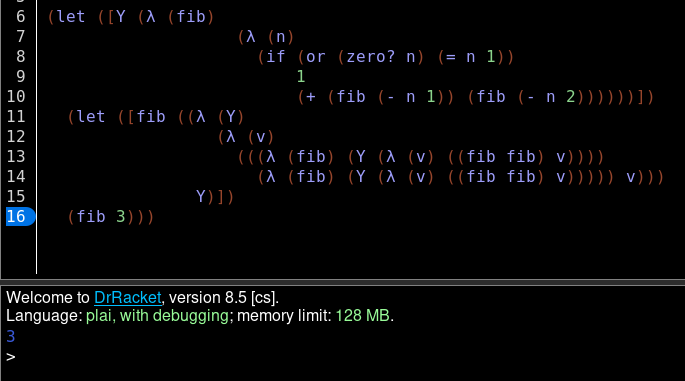
\includegraphics[scale=0.3]{./Fib-Y.png}
  \caption{Fib con combinador de punto fijo Y.}
\end{figure}

La anterior es una función \textit{mutuamente recursiva} que implementa el combinador
de punto fijo Y.  La segunda parte de la función (la que define a Y) realiza la sustitución
de punto fijo Y hasta llegar al respectivo valor y lo utiliza para no generar tantos
registros en memoría, la ejecución interna se basa en realizar las reducciones a la 2da
expresión y aplicarlas a la primera.
%%%%%%%%%%%%%%%%%%%%%%%%%%%%%      Inciso C        %%%%%%%%%%%%%%%%%%%%%%%%%%%%%%%%%
\item Modifica la función usando el Combinador de Punto Fijo Z. Prueba la expresión en 
el intérprete de \code{Racket} y con base en la respuesta obtenida, explica el proceso que 
siguió el intérprete para llegar a ésta. Anexa una captura de pantalla del intérprete 
de \code{Racket} al probar la expresión.

\begin{figure}[h]
  \centering
  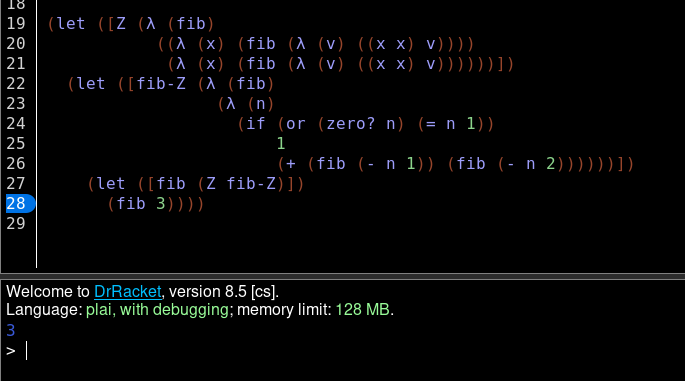
\includegraphics[scale=0.3]{./Fib-Z.png}
  \caption{Fib con combinador de punto fijo Z.}
\end{figure}

La ejecución de esta función es parecida a la anterior, pero obedece al regimen $Z(f) = f(Z(f))$
que lo que esta escrito en la línea 27 del código. La ejecución consta de las reducciones de las
lambdas que realizan recursión mutua con la función \code{fib}.
\end{enumerate}
